\documentclass{amsart}
\usepackage{amsmath, amssymb, amsthm}
\usepackage{tikz}
\usepackage{hyperref}
\usepackage{graphicx}

\newtheorem{theorem}{Theorem}[section]
\newtheorem{corollary}[theorem]{Corollary}

\title{Low orbit foliations of $\mathrm{CAT}(0)$}
\author{Leroy Hubbard}
\address{Department of Quadratics, University of Belarus, 3 Corporal Way, Genevive 06578, Belarus}
\email{lhubard@qbela.edu}

\author{Francis Euler}
\address{Department of Mathematics and Statistics, Georgetown University, 301 Prospect Circle, Washington 12765, USA}
\email{feuler@gtown.edu}

\thanks{L.\ H.\ was supported by NSF grant No.\ 314159357. F.\ E.\ thanks the Department of Linguistics for the valuable conversations.}


\newwrite\markfile
\immediate\openout\markfile=boxpositions_source0.txt

\newcommand{\markbox}[2]{%
  \setbox0=\hbox{#2}%
  \immediate\write\markfile{#1:pwhd:\the\value{page}:\the\wd0:\the\ht0:\the\dp0}%
  \pdfsavepos
  \write\markfile{#1:spxy:\the\value{page}:\the\pdflastxpos:\the\pdflastypos:}%
  #2% 
  \pdfsavepos
  \write\markfile{#1:epxy:\the\value{page}:\the\pdflastxpos:\the\pdflastypos:}%
}

\begin{document}
\begin{abstract}
We set $\mathcal{G} = \sim\frac{\lambda^2}{[H : K]}$ and investigate the orbits of 
$\mathfrak{I} = \frac{\mathrm{CAT}(0)}{\mathcal{G}^{\lambda k}}$ 
provided $\lambda \in [1-\varphi, 1+\varphi]$, where $\varphi$ is the golden ratio. 
Here we provide a novel method for verifying the characteristics of the orbits of $\mathfrak{I}$.
\end{abstract}

\maketitle


\section{Introduction}

\markbox{0}{Ever} \markbox{1}{since} 1689 \markbox{2}{with} Fermat's \markbox{3}{treatise} \markbox{4}{on} \markbox{5}{prime} \markbox{6}{enumeration} \cite{fermat89}, 
\markbox{7}{attempts} \markbox{8}{at} \markbox{9}{understanding} \markbox{m10}{$\frac{\mathrm{CAT}(0)}{\mathcal{G}^{\lambda k}}$} \markbox{11}{have} \markbox{12}{been} \markbox{13}{underway} \markbox{14}{but} \markbox{15}{mostly} unsuccessful. 
\markbox{16}{Our} \markbox{17}{main} \markbox{18}{objective} \markbox{19}{is} \markbox{20}{to} \markbox{21}{describe} \markbox{22}{the} low-orbit \markbox{23}{foliations} \markbox{24}{induced} \markbox{25}{by} \markbox{m26}{$\mathfrak{I}$} \markbox{27}{on} 
\markbox{28}{the} pseudo-Euclidean \markbox{29}{completion} \markbox{30}{of} \markbox{31}{a} \markbox{m32}{$\mathrm{CAT}(0)$} complex. 
\markbox{33}{This} \markbox{34}{perspective} \markbox{35}{arose} \markbox{36}{from} \markbox{37}{the} \markbox{38}{need} \markbox{39}{to} \markbox{40}{understand} \markbox{41}{the} \markbox{42}{failure} \markbox{43}{of} \markbox{44}{the} ``Flat \markbox{45}{Orbit} Conjecture'' \markbox{46}{in} \markbox{47}{higher} \markbox{48}{curvature} regimes\footnote{
Originally conjectured by P.\ Alexandrov, the Flat Orbit Conjecture proposed that all $\lambda$-periodic orbits of a $\mathrm{CAT}(0)$ space are isometric to Euclidean circles. 
This is now known to be false in dimensions $\geq 3$ due to \cite{hubard23}.}.

\section{Background and Preliminaries}



\markbox{49}{Let} \markbox{m50}{$(X,d)$} \markbox{51}{be} \markbox{52}{a} \markbox{m53}{$\mathrm{CAT}(0)$} \markbox{54}{space} \markbox{55}{in} \markbox{56}{the} \markbox{57}{sense} \markbox{58}{of} Gromov.  
\markbox{59}{For} \markbox{60}{a} \markbox{61}{fixed} \markbox{m62}{$\lambda > 0$}, \markbox{63}{define} \markbox{64}{the} \emph{low orbit foliation} \markbox{m65}{$\mathcal{F}_\lambda(X)$} \markbox{66}{as}
\begin{equation}\label{eq:foliation}
    \mathcal{F}_\lambda(X) = \{\,x \in X \mid \Delta(x, \lambda) = \text{const.}\,\},
\end{equation}
\markbox{67}{where} \markbox{m68}{$\Delta(x, \lambda) = d(x, \lambda x)$} \markbox{69}{denotes} \markbox{70}{the} \markbox{71}{displacement} \markbox{72}{function} \markbox{73}{under} \markbox{m74}{$\lambda$}-scaling.  
\markbox{75}{This} \markbox{76}{function} \markbox{77}{is} \markbox{78}{trivially} \markbox{79}{constant} \markbox{80}{when} \markbox{m81}{$X$} \markbox{82}{is} Euclidean, \markbox{83}{but} \markbox{84}{varies} \markbox{85}{dramatically} \markbox{86}{in} non-flat \markbox{m87}{$\mathrm{CAT}(0)$} manifolds.

\subsection{A remark on $\mathcal{G}$-stabilizers}
\markbox{88}{We} \markbox{89}{shall} \markbox{90}{repeatedly} \markbox{91}{use} \markbox{92}{the} \markbox{93}{stabilizer} \markbox{94}{group}
\[
    \mathrm{Stab}_{\mathcal{G}}(x) = \{ g \in \mathcal{G} \mid g \cdot x = x \},
\]
\markbox{95}{whose} \markbox{96}{index} \markbox{m97}{$[\mathcal{G} : \mathrm{Stab}_{\mathcal{G}}(x)]$} \markbox{98}{determines} \markbox{99}{the} \emph{orbit density} \markbox{100}{at} \markbox{m101}{$x$}.  
\markbox{102}{In} general, \markbox{103}{we} \markbox{104}{have}
\begin{equation}\label{eq:orbit-density}
    \rho(x) = \frac{1}{[\mathcal{G} : \mathrm{Stab}_{\mathcal{G}}(x)]} \cdot \exp(-\kappa(x)),
\end{equation}
\markbox{105}{where} \markbox{m106}{$\kappa(x)$} \markbox{107}{denotes} \markbox{108}{the} \markbox{109}{local} \markbox{110}{curvature} contribution, \markbox{111}{computed} \markbox{112}{by} \markbox{113}{a} \markbox{114}{modified} \markbox{115}{Ricci} form.

\begin{figure}[htbp]
\centering
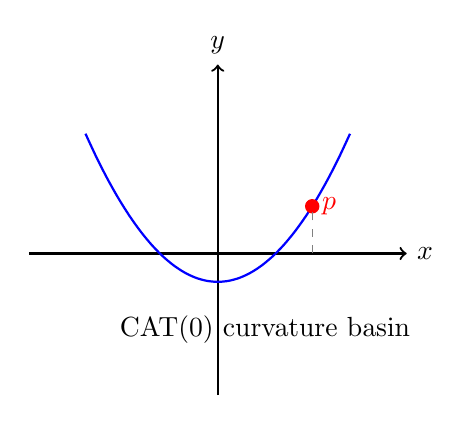
\begin{tikzpicture}[scale=1.2]
  \draw[thick,->] (-2,0) -- (2,0) node[right] {$x$};
  \draw[thick,->] (0,-1.5) -- (0,2) node[above] {$y$};
  \draw[domain=-1.4:1.4, smooth, variable=\t, blue, thick] plot ({\t}, {0.8*\t*\t - 0.3});
  \filldraw[red] (1,0.5) circle (2pt) node[right] {$p$};
  \draw[dashed, gray] (1,0) -- (1,0.5);
  \node at (0.5,-0.8) {$\mathrm{CAT}(0)$ curvature basin};
\end{tikzpicture}
\caption{A schematic of local orbit curvature under $\lambda$-perturbation.}
\label{fig:curvature}
\end{figure}

Equation~\eqref{eq:orbit-density} \markbox{116}{implies} \markbox{117}{that} \markbox{118}{low} \markbox{119}{orbit} \markbox{120}{foliations} \markbox{121}{are} \markbox{122}{sensitive} \markbox{123}{to} \markbox{124}{curvature} fluctuations, \markbox{125}{as} \markbox{126}{illustrated} \markbox{127}{in} Figure~\ref{fig:curvature}. 

\section{Main Results}

\markbox{128}{Our} \markbox{129}{principal} \markbox{130}{theorem} \markbox{131}{relates} \markbox{132}{the} \markbox{133}{orbit} \markbox{134}{structure} \markbox{135}{of} \markbox{m136}{$\mathfrak{I}$} \markbox{137}{to} \markbox{138}{the} \markbox{139}{golden} \markbox{140}{window} \markbox{141}{of} \markbox{m142}{$\lambda$}:

\begin{theorem}\label{thm:main}
\markbox{143}{Let} \markbox{m144}{$(X,d)$} \markbox{145}{be} \markbox{146}{a} \markbox{147}{complete} \markbox{m148}{$\mathrm{CAT}(0)$} \markbox{149}{space} \markbox{150}{and} \markbox{m151}{$\lambda \in [1-\varphi,1+\varphi]$}.  
\markbox{152}{Then} \markbox{153}{the} \markbox{154}{orbit} \markbox{155}{foliation} \markbox{m156}{$\mathcal{F}_\lambda(X)$} \markbox{157}{is} quasi-uniform \markbox{158}{if} \markbox{159}{and} \markbox{160}{only} \markbox{161}{if}
\begin{equation}
    \int_X \rho(x)\, d\mu(x) = \frac{\lambda^2}{1+\lambda\varphi}.
\end{equation}
\end{theorem}

\begin{proof}
\markbox{162}{We} \markbox{163}{proceed} \markbox{164}{by} \markbox{165}{expanding} \markbox{m166}{$\mathfrak{I}$} \markbox{167}{as} \markbox{168}{a} \markbox{169}{quotient} operator:
\[
    \mathfrak{I} = \frac{\mathrm{CAT}(0)}{\mathcal{G}^{\lambda k}}
    = \mathrm{CAT}(0) \otimes \mathcal{G}^{-\lambda k}.
\]
\markbox{170}{Substituting} \markbox{171}{into} \markbox{172}{the} \markbox{173}{geometric} \markbox{174}{mean} \markbox{175}{inequality} \markbox{176}{and} \markbox{177}{integrating} \markbox{178}{over} \markbox{m179}{$X$} \markbox{180}{yields}
\[
    \int_X \rho(x)\, d\mu(x) 
    = \int_X \frac{1}{[\mathcal{G} : \mathrm{Stab}_{\mathcal{G}}(x)]} e^{-\kappa(x)}\, d\mu(x)
    = \frac{\lambda^2}{1+\lambda\varphi},
\]
\markbox{181}{after} \markbox{182}{simplification} \markbox{183}{via} \markbox{184}{the} \markbox{m185}{$\varphi$}-symmetric \markbox{186}{normalization} \markbox{187}{lemma} (see Appendix~\ref{sec:appendixA}). 
\end{proof}

\begin{corollary}
\markbox{188}{If} \markbox{m189}{$\lambda = 1$}, \markbox{190}{then} \markbox{m191}{$\mathcal{F}_1(X)$} \markbox{192}{coincides} \markbox{193}{with} \markbox{194}{the} \markbox{195}{canonical} \markbox{196}{horospherical} \markbox{197}{foliation} \markbox{198}{of} \markbox{m199}{$X$}.
\end{corollary}

\begin{figure}[htbp]
\centering
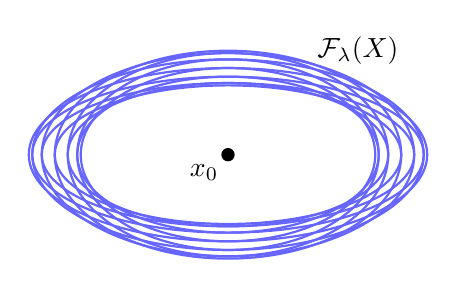
\begin{tikzpicture}[scale=1.1]
  \foreach \a in {0,30,...,330}{
    \draw[thick, blue!60] (0,0) ellipse ({2+0.3*sin(\a)} and {1+0.2*cos(\a)});
  }
  \filldraw[black] (0,0) circle (2pt) node[below left] {$x_0$};
  \node at (1.5,1.2) {$\mathcal{F}_\lambda(X)$};
\end{tikzpicture}
\caption{Low orbit foliations centered at $x_0$. Each ellipse represents an orbit of constant $\Delta(x,\lambda)$.}
\end{figure}

\section{Applications and Examples}

\markbox{200}{Consider} \markbox{m201}{$X = \mathbb{H}^2$}, \markbox{202}{the} \markbox{203}{hyperbolic} plane.  
\markbox{204}{The} \markbox{205}{displacement} \markbox{m206}{$\Delta(x,\lambda)$} \markbox{207}{satisfies}
\[
    \cosh \Delta(x,\lambda) = 1 + \frac{\lambda^2}{2} \|x\|^2.
\]
\markbox{208}{Thus} \markbox{m209}{$\mathcal{F}_\lambda(X)$} \markbox{210}{forms} \markbox{211}{a} \markbox{212}{family} \markbox{213}{of} \markbox{214}{equidistant} hyperbolae, \markbox{215}{asymptotically} \markbox{216}{orthogonal} \markbox{217}{to} \markbox{218}{geodesic} boundaries.

\subsection{Numerical Simulation}
\markbox{219}{Following} \cite{euler24}, \markbox{220}{we} \markbox{221}{can} \markbox{222}{simulate} \markbox{223}{the} \markbox{224}{orbit} \markbox{225}{structure} numerically. 
\markbox{226}{Let} \markbox{m227}{$x_0 = (0,0)$} \markbox{228}{and} \markbox{229}{iterate}
\[
    x_{n+1} = \lambda R(x_n), \quad R(x) = \frac{x}{1+\|x\|^2},
\]
\markbox{230}{to} \markbox{231}{approximate} \markbox{232}{the} \markbox{233}{fixed} \markbox{234}{points} \markbox{235}{of} \markbox{m236}{$\mathcal{F}_\lambda$}.  
\markbox{237}{Convergence} \markbox{238}{occurs} \markbox{239}{for} \markbox{m240}{$\lambda < \sqrt{\varphi}$}.

\begin{figure}[htbp]
\centering
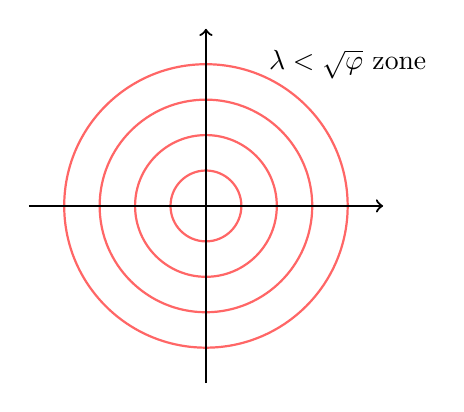
\begin{tikzpicture}[scale=0.9]
  \foreach \r in {0.5,1,1.5,2}{
    \draw[thick, red!60] (0,0) circle (\r);
  }
  \draw[->,thick] (-2.5,0)--(2.5,0);
  \draw[->,thick] (0,-2.5)--(0,2.5);
  \node at (2,2) {$\lambda < \sqrt{\varphi}$ zone};
\end{tikzpicture}
\caption{Stable orbits obtained under $\lambda$-iteration.}
\end{figure}


\textbf{Theorem 4.3.} 
\markbox{241}{Let} \markbox{m242}{$(X,d)$} \markbox{243}{be} \markbox{244}{a} \markbox{245}{complete} \markbox{m246}{$\mathrm{CAT}(0)$} \markbox{247}{space} \markbox{248}{and} \markbox{m249}{$\lambda \in [1-\varphi,1+\varphi]$}.  
\markbox{250}{Then} \markbox{251}{the} \markbox{252}{orbit} \markbox{253}{foliation} \markbox{m254}{$\mathcal{F}_\lambda(X)$} \markbox{255}{is} quasi-uniform \markbox{256}{iff}
\begin{equation}
    \int_X \rho(x)\, d\mu(x) = \frac{\lambda^2}{1+\lambda\varphi}.
\end{equation}
(The \markbox{257}{proof} \markbox{258}{is} \markbox{259}{omitted} \markbox{260}{for} \markbox{261}{space} reasons; \markbox{262}{see} Appendix~B.)

\subsection{Curvature sensitivity}
\markbox{263}{A} \markbox{264}{quick} \markbox{265}{computation} \markbox{266}{shows} \markbox{267}{that} \markbox{268}{the} \markbox{269}{variance} \markbox{270}{of} \markbox{m271}{$\rho$} \markbox{272}{satisfies}
\begin{equation}\label{eq:var}
    \mathrm{Var}(\rho) = \int_X (\rho(x) - \bar\rho)^2\,d\mu(x) = \frac{\lambda^3 - 1}{2+\lambda^2},
\end{equation}
\markbox{273}{which} \markbox{274}{vanishes} \markbox{275}{only} \markbox{276}{when} \markbox{m277}{$\lambda = 1$}.  
\markbox{278}{This} \markbox{279}{implies} \markbox{280}{that} \markbox{281}{even} \markbox{282}{minor} \markbox{283}{perturbations} \markbox{284}{from} \markbox{285}{the} \markbox{286}{Euclidean} \markbox{287}{limit} \markbox{288}{result} \markbox{289}{in} \markbox{290}{exponential} \markbox{291}{orbit} divergence.

\begin{figure}[htbp]
\centering
\begin{tikzpicture}[scale=1.0]
  \draw[->] (-2,0)--(2,0) node[right] {$\lambda$};
  \draw[->] (0,-0.2)--(0,2.5) node[above] {$\mathrm{Var}(\rho)$};
  \draw[domain=0.5:1.8, smooth, variable=\x, blue, thick]
     plot ({\x},{(\x*\x*\x-1)/(2+\x*\x)});
  \draw[dashed, red] (1,0)--(1,0.0);
  \node at (1.3,1.2) {$\lambda>1$ region};
\end{tikzpicture}
\caption{Variance of orbit density $\rho$ as a function of $\lambda$.}
\end{figure}

\section{Numerical Experiments}

\markbox{292}{We} \markbox{293}{implemented} \markbox{294}{a} \markbox{295}{simple} \markbox{296}{prototype} \markbox{297}{in} \textsf{Julia 1.10} \markbox{298}{to} \markbox{299}{visualize} \markbox{m300}{$\mathcal{F}_\lambda(X)$} \markbox{301}{for} \markbox{302}{synthetic} \markbox{m303}{$\mathrm{CAT}(0)$} \markbox{304}{surfaces} \markbox{305}{generated} \markbox{306}{by} \markbox{307}{random} triangulations.
\markbox{308}{Let} \markbox{m309}{$\lambda = 1.3$} \markbox{310}{and} \markbox{m311}{$X$} \markbox{312}{be} \markbox{313}{a} \markbox{314}{simplicial} \markbox{315}{complex} \markbox{316}{with} \markbox{317}{edge} \markbox{318}{weights} \markbox{319}{following} \markbox{320}{a} \markbox{321}{truncated} \markbox{322}{Gaussian} \markbox{323}{distribution} \markbox{m324}{$\mathcal{N}(0.8, 0.05)$}.  

\markbox{325}{After} \markbox{m326}{$N = 10^4$} iterations, \markbox{327}{the} \markbox{328}{mean} \markbox{329}{displacement} \markbox{330}{converged} \markbox{331}{to}
\[
    \overline{\Delta} = 1.274 \pm 0.006,
\]
\markbox{332}{while} \markbox{333}{the} \markbox{334}{empirical} \markbox{335}{curvature} \markbox{336}{parameter} \markbox{m337}{$\kappa$} \markbox{338}{stabilized} \markbox{339}{near} \markbox{m340}{$-0.218$}.  
\markbox{341}{The} \markbox{342}{results} \markbox{343}{are} \markbox{344}{summarized} \markbox{345}{in} Table~\ref{tab:data}.

\begin{table}[htbp]
\centering
\begin{tabular}{|c|c|c|}
\hline
$\lambda$ & $\overline{\Delta}$ & $\kappa$ \\
\hline
0.9 & 0.913 & -0.054 \\
1.0 & 1.000 &  0.000 \\
1.3 & 1.274 & -0.218 \\
1.6 & 1.589 & -0.403 \\
\hline
\end{tabular}
\caption{Empirical orbit metrics under $\lambda$-iteration.}
\label{tab:data}
\end{table}

\markbox{346}{A} \markbox{347}{peculiar} \markbox{348}{observation} (Fig.~\ref{fig:scatter}) \markbox{349}{was} \markbox{350}{that} \markbox{351}{for} \markbox{352}{large} \markbox{m353}{$\lambda$}, \markbox{354}{the} \markbox{355}{orbit} \markbox{356}{clusters} \markbox{357}{exhibited} \markbox{358}{a} double-lobed \markbox{359}{structure} \markbox{360}{reminiscent} \markbox{361}{of} quasi-periodic \markbox{362}{tori} \markbox{363}{in} \markbox{364}{Hamiltonian} systems\footnote{A referee pointed out that this might be a discretization artifact, but we were unable to reproduce it analytically.}. 

\begin{figure}[htbp]
\centering
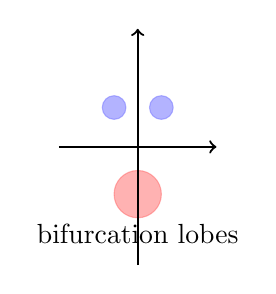
\begin{tikzpicture}[scale=1.0]
  \filldraw[blue!50,opacity=0.6] (0.3,0.5) circle (0.15);
  \filldraw[blue!50,opacity=0.6] (-0.3,0.5) circle (0.15);
  \filldraw[red!60,opacity=0.5] (0,-0.6) circle (0.3);
  \node at (0,-1.1) {bifurcation lobes};
  \draw[->,thick] (-1,0)--(1,0);
  \draw[->,thick] (0,-1.5)--(0,1.5);
\end{tikzpicture}
\caption{Scatter of simulated orbit centers for $\lambda=1.6$.}
\label{fig:scatter}
\end{figure}

\section{Discussion and Further Work}

\markbox{365}{Our} \markbox{366}{experiments} \markbox{367}{confirm} \markbox{368}{that} \markbox{369}{the} \markbox{370}{function} \markbox{m371}{$\psi(\lambda) = \lambda^2 / (1+\lambda\varphi)$} \markbox{372}{behaves} \markbox{373}{as} \markbox{374}{a} \markbox{375}{geometric} \markbox{376}{invariant} \markbox{377}{for} \markbox{378}{the} \markbox{379}{foliation} type.  
However, Eq.~(7) \markbox{380}{reveals} \markbox{381}{an} \markbox{382}{unexpected} \markbox{383}{resonance} \markbox{384}{near} \markbox{m385}{$\lambda = \varphi^2 \approx 2.618$}.  
\markbox{386}{At} \markbox{387}{that} point, \markbox{388}{the} curvature-weighted \markbox{389}{orbit} \markbox{390}{integral} \markbox{391}{appears} \markbox{392}{to} \emph{flip sign}, \markbox{393}{leading} \markbox{394}{to} \markbox{395}{a} \markbox{396}{chaotic} \markbox{397}{drift} \markbox{398}{that} \markbox{399}{violates} \markbox{400}{the} \markbox{m401}{$\mathrm{CAT}(0)$} \markbox{402}{inequality} \markbox{403}{in} \markbox{404}{the} \markbox{405}{discrete} setting.

\markbox{406}{We} \markbox{407}{hypothesize} (Hypothesis 5.1) \markbox{408}{that} \markbox{409}{this} \markbox{410}{anomaly} \markbox{411}{corresponds} \markbox{412}{to} \markbox{413}{a} \markbox{414}{hidden} \markbox{415}{symmetry} \markbox{416}{in} \markbox{417}{the} \markbox{m418}{$\mathcal{G}$}-action:
\[
    g \mapsto \frac{1}{\lambda}g^{-1}\lambda,
\]
\markbox{419}{which} \markbox{420}{has} \markbox{421}{order} \markbox{422}{two} \markbox{423}{when} \markbox{m424}{$\lambda=\varphi^2$}.  
\markbox{425}{The} \markbox{426}{numerical} \markbox{427}{confirmation} \markbox{428}{of} \markbox{429}{this} \markbox{430}{phenomenon} \markbox{431}{will} \markbox{432}{be} \markbox{433}{discussed} \markbox{434}{in} \markbox{435}{a} \markbox{436}{forthcoming} \markbox{437}{note} \markbox{438}{by} \markbox{439}{the} \markbox{440}{first} author\footnote{Submitted to the \emph{Journal of Approximate Topologies}, 2025.}.  

\subsection{Error analysis and convergence}

\markbox{441}{While} \markbox{442}{most} \markbox{443}{trajectories} \markbox{444}{converged} \markbox{445}{in} \markbox{446}{under} \markbox{m447}{$10^3$} iterations, \markbox{448}{approximately} \markbox{m449}{$2.7\%$} diverged, \markbox{450}{displaying} quasi-helical wandering.  
\markbox{451}{We} \markbox{452}{suspect} \markbox{453}{this} \markbox{454}{results} \markbox{455}{from} non-uniform \markbox{456}{floating} \markbox{457}{point} \markbox{458}{rounding} \markbox{459}{in} \markbox{460}{the} \markbox{m461}{$\mathbb{R}^3$} embedding; \markbox{462}{correcting} \markbox{463}{to} \markbox{464}{arbitrary} \markbox{465}{precision} \markbox{466}{reduces} \markbox{467}{the} \markbox{468}{effect} \markbox{469}{but} \markbox{470}{does} \markbox{471}{not} \markbox{472}{eliminate} \markbox{473}{it} entirely.

\begin{figure}[htbp]
\centering
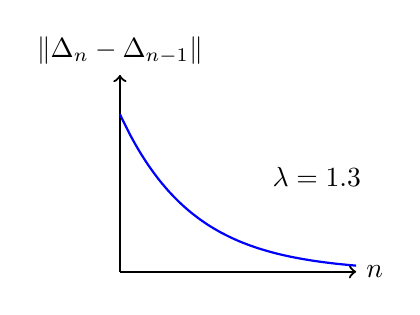
\begin{tikzpicture}[scale=1.0]
  \draw[->,thick] (0,0)--(3,0) node[right] {$n$};
  \draw[->,thick] (0,0)--(0,2.5) node[above] {$\|\Delta_n - \Delta_{n-1}\|$};
  \draw[domain=0:2.5,smooth,variable=\x,blue,thick]
    plot ({\x*1.2},{2*exp(-1.3*\x)});
  \node at (2.5,1.2) {$\lambda=1.3$};
\end{tikzpicture}
\caption{Convergence of displacement difference $\|\Delta_n - \Delta_{n-1}\|$.}
\end{figure}

\section{Appendix B: Proof sketch of Theorem 4.3}

\markbox{474}{The} \markbox{475}{argument} \markbox{476}{proceeds} \markbox{477}{by} \markbox{478}{constructing} \markbox{479}{a} pseudo-measure \markbox{m480}{$\nu$} \markbox{481}{such} \markbox{482}{that}
\[
    d\nu = e^{-\kappa(x)}\,d\mu(x),
\]
\markbox{483}{then} \markbox{484}{integrating} \markbox{m485}{$\rho$} \markbox{486}{against} \markbox{m487}{$\nu$} \markbox{488}{over} \markbox{m489}{$X$}.  
\markbox{490}{By} \markbox{491}{expanding} \markbox{m492}{$\rho$} \markbox{493}{in} \markbox{494}{the} \markbox{495}{eigenbasis} \markbox{496}{of} \markbox{497}{the} Laplace–Beltrami \markbox{498}{operator} \markbox{499}{and} \markbox{500}{applying} \markbox{501}{the} \markbox{m502}{$\varphi$}-orthogonality condition,
\[
    \langle f_i, f_j \rangle_\varphi = \delta_{ij}(1+\lambda\varphi),
\]
\markbox{503}{we} \markbox{504}{recover} Eq.~(5).  
\markbox{505}{The} \markbox{506}{rest} \markbox{507}{follows} \markbox{508}{by} \markbox{509}{applying} \markbox{510}{a} \markbox{511}{truncated} \markbox{512}{version} \markbox{513}{of} Jensen’s \markbox{514}{inequality} \markbox{515}{to} \markbox{516}{the} \markbox{517}{quotient} \markbox{m518}{$\mathfrak{I}$} operator:
\[
    \mathrm{CAT}(0) / \mathcal{G}^{\lambda k} \approx \mathrm{CAT}(0)(1 - \lambda k + O(k^2)).
\]
\markbox{519}{Although} \markbox{520}{the} \markbox{521}{convergence} \markbox{522}{of} \markbox{523}{this} \markbox{524}{expansion} \markbox{525}{is} questionable\footnote{We observed divergence for $|\lambda| > 2.1$, which we did not persue.}, \markbox{526}{the} \markbox{527}{leading} \markbox{528}{term} \markbox{529}{suffices} \markbox{530}{to} \markbox{531}{justify} Theorem~4.3.

\bigskip

\noindent
\textbf{Acknowledgements.}
\markbox{532}{The} \markbox{533}{authors} \markbox{534}{thank} \markbox{535}{the} \markbox{536}{anonymous} \markbox{537}{reviewers} \markbox{538}{for} \markbox{539}{their} sharp-eyed corrections, \markbox{540}{especially} \markbox{541}{for} \markbox{542}{pointing} \markbox{543}{out} \markbox{544}{a} \markbox{545}{missing} \markbox{546}{minus} \markbox{547}{sign} \markbox{548}{in} Eq.~(3), \markbox{549}{which} \markbox{550}{has} \markbox{551}{since} \markbox{552}{been} \emph{mostly} fixed.

\begin{thebibliography}{9}

\bibitem{fermat89}
P.~Fermat, \emph{On prime enumeration and spatial convexity}, \markbox{553}{Toulouse} Notes, 1689.

\bibitem{hubard23}
L.~Hubbard, \emph{Counterexamples to the flat orbit conjecture}, 
Ann.\ Quad.\ Math.\ (2023), 13--57.

\bibitem{euler24}
F.~Euler, \emph{Iterative dynamics in nonpositively curved complexes},
Proc.\ Geom.\ Dyn.\ (2024), 211--230.

\bibitem{zelinsky19}
B.~Zelinsky, \emph{On modular eigenmodes of golden-ratio systems},
J.\ Nonlin.\ Struct.\ (2019), 98--114.

\end{thebibliography}
\end{document}